\documentclass[12pt,margin=0px]{article}

\usepackage[a4paper, margin=1in]{geometry}
\usepackage[export]{adjustbox}
\usepackage[hungarian]{babel}
\usepackage[normalem]{ulem}
\usepackage[table,xcdraw]{xcolor}
\usepackage[thinlines]{easytable}
\usepackage[utf8]{inputenc}
\usepackage{amsmath}
\usepackage{amssymb}
\usepackage{amsthm}
\usepackage{enumitem}
\usepackage{fancyhdr}
\usepackage{float}
\usepackage{fontawesome}
\usepackage{geometry}
\usepackage{graphicx}
\usepackage{hhline}
\usepackage{ifthen}
\usepackage{listings}
\usepackage{makecell}
\usepackage{multirow}
\usepackage{newunicodechar}
\usepackage{pgf,tikz}
\usepackage{subcaption}
\usepackage{tipa}
\usepackage{wasysym}
\usepackage{xcolor}
\usetikzlibrary{positioning,calc,shapes.multipart,arrows,arrows.meta,matrix,automata}

 \geometry{
 a4paper,
 total={170mm,297mm},
 left=20mm,
 right=20mm,
 top=20mm,
 bottom=20mm
 }

\renewcommand{\figurename}{ábra}
\newenvironment{tetel}[1]{\paragraph{#1 \\}}{}
\renewcommand{\baselinestretch}{1.15}

\newcommand{\N}{\mathbb{N}}
\newcommand{\Z}{\mathbb{Z}}
\newcommand{\R}{\mathbb{R}}
\newcommand{\Q}{\mathbb{Q}}
\newcommand{\C}{\mathbb{C}}

\definecolor{mygray}{rgb}{0.0, 0.0, 0.0}
\definecolor{blue(pigment)}{rgb}{0.2, 0.2, 0.6}
\definecolor{brickred}{rgb}{0.8, 0.25, 0.33}
\definecolor{coolblack}{rgb}{0.0, 0.18, 0.39}

\setlist[itemize,1]{label=$\bullet$}
\setlist[itemize,2]{label=$\circ$}
\setlist[itemize,3]{label=$\centerdot$}
\setlist[itemize,4]{label=$\bullet$}

% A dokument itt kezdődik

\date{}
\useunder{\uline}{\ul}{}
\fancyhf{} % sets both header and footer to nothing
    \lfoot{ELTE-IK}
    \cfoot{\thepage}
    \rfoot{6. tétel }

\pagestyle{fancy}

\renewcommand{\headrulewidth}{0pt}
\renewcommand{\footrulewidth}{0.4pt}

\begin{document}
    \hyphenation{oddword}
    \uchyph=0
    \begin{center}
        {\Large\bfseries\noindent 6. Mesterséges intelligencia} \\
    \end{center}

	\section*{Bevezetés}
	
	\noindent Az MI az intelligens gondolkodás számítógépes reprodukálása szempontjából hasznos elveket, módszereket, technikákat kutatja, fejleszti, rendszerezi.\\\\
    Megoldandó feladatai
    \begin{itemize}
        \item nehezek, mert ezek problématere hatalmas,
        \item a megoldás megkeresése kellő intuíció hiányában kombinatorikus robbanáshoz vezethet.
        \begin{itemize}
            \small \color{mygray}
            \item Például az utazó ügynök probléma $n$ város esetén $(n-1)!$ a lehetséges utak (élek) száma. Ebben az esetben az alaphalmaz elemeinek kis mértékű változása is már exponenciális mértékben nőveli a problématér elemeinek számát.
            \begin{itemize}
                \item $n = 5$ esetén, $4! = 24$
                \item $n = 50$ esetén, $49! \sim 6 * 10^{62}$
            \end{itemize}
        \end{itemize}
    \end{itemize}
    A szoftver intelligensen viselkedik, és sajátos eszközöket használ. A reprezentáció átgondolt a feladat modellezéséhez, és az algoritmusok hatékonyak, heurisztikával megerősítve.
	
	\section*{Útkeresési problémák}

    \noindent Útkeresési problémaként sok MI feladat fogalmazható meg úgy, hogy a feladat modellje alapján megadunk egy olyan élsúlyozott irányított gráfot, amelyben adott csúcsból adott csúcsba vezető utak jelképezik a feladat egy-egy megoldását. Ezt a feladat \textbf{\textit{gráfreprezentációjának}} is szokás nevezni, amely magába foglal egy úgynevezett \textbf{\textit{$\delta$-gráfot} (delta gráf)} (olyan élsúlyozott irányított gráf, ahol egy csúcsból kivezető élek száma véges, és az élek költségére megadható egy $\delta$ pozitív alsó korlát), az abban kijelölt startcsúcsot és egy vagy több célcsúcsot. Ebben a reprezentációs gráfban keresünk egy startcsúcsból kiinduló célcsúcsba futó utat, esetenként egy legolcsóbb ilyet.\\

    {\footnotesize \noindent {\color{blue} \faLightbulbO\ $\triangleright$ } }

    {\footnotesize
    \noindent Legyen az $(N,A,c)$ egy él-súlyozott irányított gráf, amely csúcsainak halmaza az $N$, éleinek halmaza az $A\subseteq N \times N$, az $(n,m) \in A$ egy $n$ csúcsból $m$ csúcsba irányuló élt jelöl (az él kiinduló csúcsát szülőnek, végcsúcsát gyereknek szokták hívni), a $c: A \rightarrow R$ pedig az élekhez súlyt (a továbbiakban költséget) rendelő függvény.
    }\\

    {\footnotesize
    \noindent A szokásoktól némileg eltérően itt feltételezzük, hogy az irányított gráfokban akár \textbf{végtelen sok csúcs} is lehet. Ez abból adódik, hogy a vizsgált feladatok problématerének mérete nagyon nagy, sőt esetenként valóban végtelen. Az informatikai megoldások szempontjából viszont nincs különbség a végtelen és a nagyon nagy méret között: az olyan algoritmusok úgysem használhatók, amelyek arra rendezkednek be, hogy megvizsgálják a teljes problémateret.
    }\\

    {\footnotesize
    \noindent A fentiek természetes következménye, hogy gráfjainkban végtelen sok irányított él fordulhat elő. Kikötjük azonban azt, hogy egy csúcsból kivezető élek száma legyen véges, azaz mindegyik csúcsnak csak \textbf{véges sok gyereke} van. (Egy csúcshoz azonban tartozhat végtelen sok szülőcsúcs.) Ez a megszorítás nem jelent valódi korlátozást, mert a kivezető éleket általában a megoldandó feladathoz definiált műveleteket generálják. Egy adott pillanatban alkalmazható műveletek száma pedig egy valós feladat esetében mindig véges. Ráadásul a műveletek pozitív végrehajtási költséggel rendelkeznek – már ha egyáltalán számít a végrehajtási költségük –, és megfigyelhető, hogy a műveletek költségeinek infinuma is egy pozitív szám. Így azt is kiköthetjük, hogy az él-súlyozott irányított gráfjaink élsúlyai (élköltségei) egy, a teljes gráfra érvényes pozitív valós számnál nem kisebbek. Ezt a súlykorlátot gyakran szokták a görög $\delta$ betűvel jelölni, az általa leírt tulajdonságot pedig \textbf{$\delta$-tulajdonságnak} hívni. (Az élek súlyait egységesen egységnyinek tekintjük akkor, amikor a megoldandó feladatban semmilyen utalás sincs a költségekre.)
    }\\

    {\footnotesize
    \noindent Egy végtelen sok csúcsból álló, de egy csúcshoz csak véges sok kivezető élt rendelő, $\delta$-tulajdonságú $(N,A,c)$ él-súlyozott irányított gráfot röviden \textbf{$\delta$-gráfnak} szoktunk nevezni. Egy útkeresési feladat egy $\delta$-gráfbeli bizonyos tulajdonságú irányított út megkeresését jelenti.
    }\\

    {\footnotesize
    \noindent Egy $n \in N$ csúcsból $m \in N$ csúcsba vezető irányított úton egy $<(n,n_1), (n_1,n_2), \cdots , (n_{k-1},m)>$ él-sorozatot értünk.
    }\\

    {\footnotesize
    \noindent Egy irányított út hosszán az utat alkotó élek számát értjük, és egy $\alpha$ út esetében az $\alpha$ szimbólummal jelöljük. Az $\alpha = <(n_0,n_1), (n_1,n_2), ... , (n_{k-1},n_k)>$ út költségét a $c\alpha(n_0,n_k)$, vagy röviden a $c(\alpha)$ szimbólum jelöli majd, amelyet – a hosszúság fogalmához illeszkedően – az utat alkotó élek költségeinek összegeként definiáljuk:
    }
    \[
        c(\alpha) = \sum_{i=1}^{k}c(n_{i-1},n_{i})
    \]

    {\footnotesize
    \noindent A $\delta$-gráfokban, amennyiben vezet egy csúcsból ($n$) egy csúcshalmazba ($M$) út, akkor létezik ezek között legrövidebb út is, sőt legolcsóbb költségű, azaz optimális út is.
    }\\

    {\footnotesize
    \noindent Bevezetjük a $c^{*}:N \times N \rightarrow R$ függvényt, amely egy $\delta$-gráfban megadja azt az optimális (legolcsóbb) költséget, amely árán egy csúcsból egy másikba el lehet jutni. Ezt mindegyik n és m csúcsra értelmezzük: ha létezik { $n \rightarrow m$ }-beli út, akkor ezek költségeinek minimumaként; ha nem létezik, akkor végtelen nagynak tekintjük. Formálisan:
    }
    \[
        c^{*}(n, m) = \left\{ \begin{array}{cc}
                               min_{\alpha \in {n \rightarrow m}}c(\alpha) & ha\ \exists n \rightarrow m \\
                               \infty & ha\ \not\exists n \rightarrow m
                             \end{array}
         \right.
    \]
    {\footnotesize
    \noindent Egy útkeresési feladat modellezésekor az a célunk, hogy a feladat problématerét egy $\delta$-gráfbeli, adott csúcsból (startcsúcsból) induló irányított utak halmazaként fogalmazzuk meg, amelyek között olyan utat keresünk, amely adott csúcsok (célcsúcsok) egyikébe vezet. Gyakran az optimális út megtalálása a célunk. Ennek megfelelően egy útkeresési feladat \textbf{gráfreprezentációján} azt értjük, ha megadunk egy $(N,A,c)$ $\delta$-gráfot, az úgynevezett \textbf{reprezentációs gráfot}, kijelöljük annak $s \in N$ startcsúcsát és $T \subseteq N$ célcsúcsait. A feladat általánosan az, hogy egy $s \rightarrow T$-beli úgynevezett \textbf{megoldási utat} (vagy röviden megoldást) kell megtalálnunk, esetenként egy $s \rightarrow^{*}T$-beli \textbf{optimális megoldási utat} (az optimális megoldást).}\\
    \noindent {\footnotesize $\triangleleft$ \faLightbulbO }

	\section*{Állapottér-reprezentáció}

    \noindent Az állapottér reprezentáció egy általános probléma-modellezési módszer, amellyel részletesen specifikálhatjuk a megoldandó feladatot úgy, hogy azt útkeresési feladattá fogalmazzuk át. Ez által lehetővé válik, hogy a problémára úgy tekinthessünk, mint egy $\delta$-gráfbeli út keresésére.\\
    {\small \color{mygray}Mivel ennek során arról is döntünk, hogy a feladatból kinyert ismereteket milyen formában rögzítsük a számítógépen, ezért az állapottér specifikáció helyett az \emph{állapottér reprezentáció} szóhasználat terjedt el.}\\

    \noindent Az állapottér reprezentációnak négy fő eleme van:
	\begin{itemize}
	   \item \textit{Állapottér}: A probléma leírásához szükséges adatok által felvett érték-együttesek (állapotok) halmaza. Az állapot többnyire összetett szerkezetű érték (osztály vagy stuktúra). Gyakran egy bővebb alaphalmazzal és egy azon értelmezett invariáns állítással definiáljuk.
		\item \textit{Műveletek}: A műveletek az állapottéren definiált, azaz állapothoz állapotot rendelő operátorok, amelyek értelmezési tartománya jelöli ki azt, hogy mely állapotokra hajthatók végre. Megadásukhoz szükséges az előfeltétel és hatás leírása, valamint az invariáns tartó leképezés.
		\item \textit{Kezdőállapot(ok)} A feladat lehetséges kezdő állapotai megadhatóak közvetlenül, vagy közvetve egy logikai állítás (a kezdő feltétel) segítségével. A feladat egy konkrét kitűzéséhez mindig egy konkrét kezdő állapotot kell meghatároznunk.
		\item \textit{Célállapot(ok)}. Egy adott kezdő állapothoz tartozó célállapot (vagy célállapotok) megadható közvetlenül, vagy közvetve egy logikai állítás segítségével.
	\end{itemize}

    {\footnotesize \noindent {\color{blue} \faLightbulbO\ $\triangleright$ }

    \noindent Az objektum elvű programozási paradigma értelmében a definíció első két pontja egy adattípust (egy osztályt) definiál. A műveletek (metódusok) az osztály egy objektumára hajthatóak végre, amelynek állapota ennek hatására megváltozik. A számítógépes megvalósításoknál az objektum kezdő állapotát a konstruktor, vagy egy speciális inicializáló metódus állítja be, a célfeltételt pedig egy logikai értéket visszaadó metódus ellenőrzi.}\\

    {\footnotesize
    \noindent Az állapottér reprezentáció lehetőséget teremt arra, hogy a megoldandó problémának elkészítsük a gráfreprezentációját, amelyben a probléma már nyilvánvalóan útkeresési feladattá válik. Minden állapottér reprezentációnak megfeleltethető egy irányított élsúlyozott gráf, amelyben kijelölhetünk egy startcsúcsot és egy vagy több célcsúcsot. Egy állapottér reprezentáció \textbf{állapot gráfjának} nevezzük azt a $\delta$-gráfot, amelyben a csúcsok az állapotokat, az élek a műveletek végrehajtásait, azaz az állapot-átmeneteket szimbolizálják, az élek súlyai a megfelelő műveletek költségei lesznek, ezek hiányában egységesen egységnyi az értékük. Az állapottér reprezentációval leírt feladat egy konkrét kitűzésében szereplő kezdőállapotot megjelenítő csúcsot hívjuk startcsúcsnak ($s$), kezdőállapothoz tartozó célállapot(ok)nak megfeleltetett csúcso(ka)t célcsúcs(ok)nak ($T$). (Vegyük észre, hogy a gráfreprezentáció önmagában nem egy külön feladat modellező módszer, hanem csak az eredménye egy probléma modellezésnek.)
    }\\
    \newpage
    {\footnotesize\noindent Példa: n-királynő probléma állapottér reprezentációja}\\

    {\footnotesize
    \noindent State = rec(board: Board, count : $\mathbb{N}$)\\\\
    Board=$\Big\{$
        \begin{itemize}
            \item[] $a \in \{
\includegraphics[width=0.0225\linewidth]{img/queen.png}, \boxtimes , \square\}^{n \times n}$,
            \item[] $a.count \in [0 \ldots n]\ \wedge$
            \item[] $\forall i \in [1\ \ldots\ a.count]: Count(a,\ i)=1\ \wedge$
            \item[] $\forall i \in [a.count + 1\ \ldots\ n]: Count(a,\ i)=0$
        \end{itemize} $\Big\}$\\\\
    Move(column): $State \ \rightarrow\ State\qquad (column \in [1 \ldots n],\ act \in State)$\\
    IF $(act.count < n) \wedge (act.board[act.count + 1,\ column] \neq \boxtimes)$\\
    THEN\\
        $act.count := act.count+1\ :\ act.board[act.count,\ column] := 
\includegraphics[width=0.0225\linewidth]{img/queen.png}$\\
        $\forall i,\ j: $\\
        IF ($act.board[i,\ j].threatenBy(
\includegraphics[width=0.0225\linewidth]{img/queen.png})\ \wedge\ (act.board[i,\ j]\ == \square)$\\
        THEN\\
        $act.board[i,\ j] := \boxtimes$
    }
	\begin{figure}[H]
		\centering
		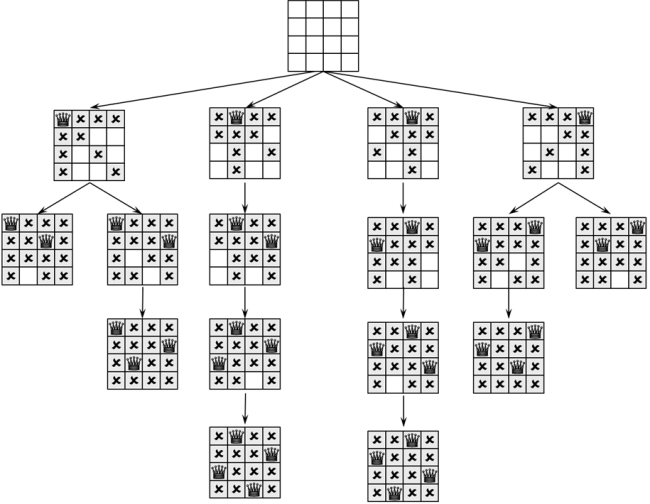
\includegraphics[width=0.48\linewidth]{img/four_queen_problem_sample.png}
		\caption{A 4-királynő probléma állapot gráfja.}
		\label{fig:fourqueen_sample}
	\end{figure}
	
    \color{mygray} \subsubsection*{Állapottér modell - Állapot-gráf}
    \renewcommand{\arraystretch}{2}
    {\noindent \footnotesize \color{mygray}
    \begin{tabular}{lcl}
      \hline
       \textbf{Állapottér modell}               &  & \textbf{Állapot-gráf}
       \\
       \textit{ - állapot}                         & $\sim$ & \textit{csúcs}
       \\
       \textit{ - művelet hatása egy állapotra}    & $\sim$ & \textit{irányított él}
       \\
       \textit{ - művelet költsége}                & $\sim$ & \textit{él költsége}
       \\
       \textit{ - kezdő állapot}                   & $\sim$ & \textit{startcsúcs}
       \\
       \textit{ - célállapot}                      & $\sim$ & \textit{célcsúcs}
       \\
       \textbf{Gráf-reprezentáció}              &  & \textit{állapotgráf, startcsúcs, célcsúcsok}
       \\
       \textit{ - egy műveletsorozat hatása}       & $\sim$ & \textit{irányított út}
       \\
       \textit{ - megoldás}                        & $\sim$ & \textit{irányított út a startcsúcsból egy célcsúcsba}
       \\ \hline
    \end{tabular}
    \renewcommand{\arraystretch}{1}}\\\\\\
    \noindent Egy feladat állapottér modellje és problématere között szoros kapcsolat áll fenn, de az állapottér nem azonos a problématérrel. A problématér elemeit (lehetséges megoldásokat) a gráf reprezentációbeli startcsúcsból induló különböző hosszúságú irányított utak szimbolizálják.\\
	{\footnotesize $\triangleleft$ \faLightbulbO}

	\section*{Kereső-rendszerek}
	
    Azok a kereső algoritmusok, amelyek egy reprezentációs gráfban ($\delta$-gráfban) keresnek $s \rightarrow T$-beli utat az alapvető különbségeik ellenére egy közös ősből származtathatóak. Ezt hívjuk \emph{kereső rendszernek}.

	\subsubsection*{\textit{Általános keresőrendszer} részei}

    \begin{itemize}
        \item \textit{{Globális munkaterület}} (a keresés memóriája)
        \item \textit{{Keresési szabályok}} (a memória tartalmát változtatják meg)
        \item \textit{{Vezérlési stratégia}} (adott pillanatban alkalmas szabályt választ)
        \begin{itemize}
            \item \emph{Általános}: független a feladattól és annak modelljétől.
            \begin{itemize}
                {\small
                \color{mygray}
                \item nem módosítható
                \item módosítható}
            \end{itemize}
            \item \emph{Modellfüggő}: nem függ a feladat ismereteitől, de épít a feladat modelljének általános elemeire.
            \item \emph{Heurisztikus}: a feladattól származó, annak modelljében nem rögzített, a megoldást segítő ismeret, amelyet közvetlenül a vezérlési stratégiába építünk be az eredményesség és a hatékonyság javítása céljából.
	   \end{itemize}
    \end{itemize}

    {\footnotesize
    \noindent {\color{blue} \faLightbulbO\ $\triangleright$ }
    \begin{itemize}
        \item \textit{{Globális munkaterület}} A globális munkaterület annak az információnak a tárolására szolgál, amelyet a rendszer a keresés során megszerez, és megőrzésre fontosnak ítél. Egy $\delta$-gráfban történő keresésnél ez a gráfnak az a startcsúcsból elérhető része, amelyet a keresés felfedezett és megjegyzett. Ez lehet csak egyetlen csúcs, esetleg annak környezete, lehet egy út, amelyik a startcsúcsból az aktuálisan vizsgált csúcsba vezet, de lehet egy ennél tágabb részgráf is. A globális munkaterület minden keresés esetén rendelkezik valamilyen kezdeti értékkel, amely általában a startcsúcs. Akkor terminál, ha a globális munkaterület kielégíti a terminálási feltételt, amely egy célcsúcsnak a globális munkaterületen való megjelenésével kapcsolatos.
        \item \textit{{Keresési szabályok}}: A kereső rendszer minden lépésben egy kereső szabály által változtatja meg a globális munkaterületet. A kereső szabály tehát a munkaterület operátora. Minden szabály rendelkezik egy előfeltétellel (ez határozza meg a szabály értelmezési tartományát) és egy hatással (amelyet a végrehajtásakor kifejt). Egy $\delta$-gráfban folyó keresésnél ez például új csúcsra cserélheti a globális munkaterületen tárolt csúcsot, vagy új élt fűzhet hozzá a munkaterületen levő úthoz.
        \item \textit{{Vezérlési stratégia}} Egy adott pillanatban több végrehajtható kereső szabály is lehet. A vezérlési vagy keresési stratégia feladata ezek közül egyet kiválasztani. Amíg a globális munkaterületen és a kereső szabályokban a megoldandó feladat reprezentációjában rögzített ismeretei jelennek meg, addig a vezérlési stratégia a reprezentációtól független összetevője a kereső rendszernek. A stratégia megválasztását természetesen befolyásolja a megoldandó feladat, és a feladat reprezentálásához választott módszer, de a konkrét feladat reprezentációja nincsen rá hatással. Ugyanakkor a vezérlési stratégia megválasztása kihat a kereső rendszer többi komponensére is.\\
    \end{itemize}
    A vezérlési stratégia három szintre tagolható:
    \begin{itemize}
                \item Az \textbf{\emph{elsődleges vezérlési stratégia}} (általános) teljesen független a megoldandó feladattól. Ezen a szinten nem módosítható és módosítható stratégiákat különböztethetünk meg. Az előbbiek azok, amelyek alkalmazásakor egy kiválasztott kereső szabály végrehajtása végleges, vissza nem vonható; az utóbbi alkalmazása során ellenben lehetőségünk van korrigálásra.
                \item A \textbf{\emph{másodlagos vezérlési stratégia}} (modelfüggő) a megoldandó feladattól független ugyan, de függ a feladat reprezentálásához választott modelltől. Mivel ebben a jegyzetben csak egyféle modell szerepel (az állapottér reprezentáció), amelyhez viszont nem kapcsolódik jellegzetes másodlagos vezérlési stratégia, ezért erre itt nem tudunk példát mutatni.
                \item A MI feladatainál a problématér olyan nagy, hogy nem szerencsés, ha a feladatokat csupán "vak" kereséssel, minden lehetséges utat szisztematikusan végig próbálva kíséreljük meg megoldani. Az ilyen módszer általában kombinatorikus robbanáshoz, azaz kezelhetetlenül nagy adattömeghez vezet. Egy keresés csak akkor lehet sikeres, ha a vezérlési stratégiájába olyan – a feladatból származó többlet – ismeretet épít be, amely korlátozni képes keresést úgy, hogy a lehetséges folytatások közül csak ígéretesekkel foglalkozzon. Ez a speciális vezérlési ismeret, az úgynevezett \emph{\textbf{heurisztika}}, a vezérlési stratégiák harmadik szintje. E nélkül a feladat megoldása még a mai számítógépek működési sebessége és memória kapacitása mellett is reménytelen.\\

                    Megkülönböztetjük tehát a feladattal kapcsolatos ismereteket aszerint, hogy azokat a reprezentációban deklaratív módon (azaz a globális munkaterületen) illetve procedurális módon (a kereső szabályokban) használjuk-e fel, vagy vezérlési ismeretként a stratégiát javítjuk-e általa. A heurisztikára úgy tekintünk, mint a feladattal kapcsolatos olyan információra, amit nem a reprezentációban rögzítünk, hanem közvetlenül az algoritmusba építünk be. A heurisztika feladata, hogy pontosítsa azt alkalmazható kereső szabályok közötti sorrendet, amelyet elsődlegesen, a feladattól függetlenül a vezérlés jelöl ki. A heurisztika a vezérlési stratégia finomítását, a mindenkori feladatra történő ráhangolását végzi.\\

                    A heurisztika alkalmazásától azt várjuk, hogy javítsa a keresés eredményességét, azaz találjon megoldást, esetleg jó minőségű megoldást, továbbá javítsa a keresés hatékonyságát. A heurisztikát alkalmazó keresések tulajdonságait az alábbiak szerint fogalmazhatjuk meg:
                    \begin{itemize}
                        \item a legtöbb esetben "elég jó" megoldást találnak, bár nem garantálnak optimális megoldást, sőt valójában semmiféle megoldást nem garantálnak.
                        \item jelentős mértékben javítják a problémamegoldó program hatékonyságát, főként a keresés próbálkozásai számának csökkentésével.
                    \end{itemize}
   \end{itemize}
    $\triangleleft$ \faLightbulbO}

	\subsection*{Lokális keresés}

	\begin{itemize}
    	\item A lokális keresések egyetlen aktuális csúcsot és annak szűk környezetét tárolják a globális munkaterületen.
        \begin{itemize}
            {\small
            \color{mygray}
            \item Kezdetben az aktuális csúcs a startcsúcs, és a keresés akkor áll le, ha az aktuális csúcs a célcsúcs lesz, vagy ha nem tud továbblépni.}
        \end{itemize}
        \item Keresési szabályai az aktuális csúcsot minden lépésben a szomszédjai közül vett lehetőleg  ,,jobb” gyerekcsúccsal cserélik le.
        \item A vezérlési stratégiájuk a ,,jobbság” eldöntéséhez egy \textit{rátermettségi függvényt} használ, amely annál jobb értéket ad egy csúcsra, minél közelebb esik az a célhoz.
        \begin{itemize}
            \item Ez egy \textit{nem-módosítható vezérlési stratégia}, mivel a keresés ,,elfelejti”, hogy honnan jött, így a döntések nem vonhatók vissza.
        \end{itemize}
    \end{itemize}
	\emph{Lokális kereséssel megoldható feladatok} azok, ahol egy lokálisan hozott rossz döntés nem zárja ki a cél megtalálását. Ehhez vagy egy erősen összefüggő reprezentációs-gráf, vagy jó heurisztikára épített
	célfüggvény kell. Jellemző alkalmazás:  Adott tulajdonságú elem keresése, vagy például függvény optimumának keresése.\\

    {\footnotesize
    \noindent {\color{blue} \faLightbulbO\ $\triangleright$ }

    {\footnotesize
    \noindent A lokális keresések úgy próbálnak megoldási utat találni egy reprezentációs gráfban, hogy a keresés során a gráfnak csak egy csúcsát (az úgynevezett aktuális csúcsot) és annak környezetét (például a gyerekeit, szülőjét, esetleg visszamenőleg néhány ősét) ismerik. Ezen korlátozott ismeretek alapján döntenek arról, hogy az aktuális csúcsot annak melyik gyerekére cseréljék le. Ennek kiválasztásához nélkülözhetetlen egy heurisztikus függvény, az úgynevezett célfüggvény. Ez az aktuális csúcs gyerekeihez rendel olyan értékeket, amelyek alapján eldönthetjük, hogy melyik a legígéretesebbnek látszó gyerekcsúcs.
    }\\

    {\footnotesize
    \noindent A lokális keresések nem-módosítható vezérlési stratégiát használó kereső rendszerek. Globális munkaterületükön az aktuális csúcsot (kezdetben a startcsúcsot) és annak környezetében levő csúcsokat tárolják. Kereső szabályaik az aktuális csúcsot cserélik annak környezetéből vett másik csúcsra (többnyire valamelyik gyerekére) és ezzel egyidejűleg módosítják az aktuális csúcs környezetéről nyilvántartott ismereteket. Több lehetőség esetén az adott pillanatban lehető legjobbnak látszó csúcsot választják új aktuális csúcsnak, azaz egyfajta mohó stratégiát követnek. A továbblépésnél hozott döntéseik visszavonhatatlanok (nem módosíthatóak), nem áll módjukban a döntéseiket meg nem történtté tenni, és új döntést hozni. Sikeres terminálás (azaz célcsúcs elérése) esetén nem képesek a megoldási utat visszaadni, csak ha működésük közben folyamatosan naplózzák (rögzítik) azt, hogy mely csúcsokat érintették a keresés során.
    }\\

    {\footnotesize
    \noindent A lokális keresések csak speciális esetekben alkalmazhatók sikerrel az MI feladatok megoldására. Vagy a döntéseknél felhasznált célfüggvénynek, a heurisztikának kell elég erősnek lennie ahhoz, hogy csalhatatlanul a megfelelő irányba vezesse a keresést, vagy a reprezentációs gráfnak kell olyan alakúnak lenni, hogy egy-egy rossz döntés ne veszélyeztesse a célcsúcs elérését. Heurisztika ez utóbbi esetben is szükséges ahhoz, hogy a keresés eredményes és gyors legyen.
    }\\

    {\footnotesize
    \noindent A lokális keresés alkalmazása kifejezetten előnytelen akkor, ha a reprezentációs gráf egy irányított fa (lásd n-királynő probléma vagy utazó ügynök probléma), mert kizárólag tökéletes heurisztikájú célfüggvény esetén lehet sikeres.
    }\\
    $\triangleleft$ \faLightbulbO}

    \subsubsection*{Lokális keresést megvalósító algoritmusok}

	\begin{itemize}
		\item \textit{\textbf{Hegymászó algoritmus}}: A legyegyszerűbb lokális keresési algoritmus.
        \begin{itemize}
            \item A \emph{globális munkaterületén} nyilvántartja:
            \begin{itemize}
                \item az aktuális csúcsot ($akt$), és
                \item az $akt$ csúcs szülőjét $\pi(akt)$
            \end{itemize}
            \item A keresési szabálya:
            \begin{itemize}
                \item előállítja az $akt$ csúcs gyermek csúcsait,
                \item a cél elérése szempontjából leígéretesebb csúcsra lép, kizárva a szülő való visszalépést.\\
                (Az algoritmusban feltételezzük azt, hogy egy csúcs annál ígéretesebb, minél kisebb annak célfüggvény ($f$) értéke.)
            \end{itemize}
            \item \emph{Hátrányai}:
                \begin{itemize}
                    {\small
                    \item Csak erős heurisztika esetén lesz sikeres, ennek hiányában gyakorta rossz, nem a cél irányába mutató döntést fog hozni, amely következtében akár véglegesen tévútra kerülhet. Általában egy reprezentációs gráf tartalmazhat olyan részeket, ahonnan már nem vezet út célcsúcsba. Ha a heurisztika ilyen helyre navigálja a keresést, akkor az már nem lehet eredményes. A hegymászó módszer tehát nem garantálja a megoldás megtalálását.
                    \item A módszer lokális optimum hely környezetében és ekvidisztans felületen (azonos célfüggvény értékű szomszédos csúcsok körzetében) eltévedhet. A keresést ugyanis ilyenkor nem irányítja a célfüggvény, véletlenszerűen kell új aktuális csúcsot választani, és mivel a keresés nem végezhet körfigyelést (nem tárolja a korábban bejárt csúcsokat) könnyen végtelen ciklusba eshet.
                    \item A keresés zsákutcába (olyan csúcs, amelynek nincsenek gyerekei) jutva beragad.
                    }\\
                \end{itemize}
        \end{itemize}
        \newpage
		\item \textit{\textbf{Tabu keresés}}: Algoritmus a  hegymászó algoritmus kis memóriájából származó hátrányok kiküszöbölésére.
        \begin{itemize}
            \item A \emph{globális munkaterületén} nyilvántartja:
            \begin{itemize}
                \item az aktuális csúcsot ($akt$), és
                \item az eddig legjobbnak bizonyult csúcsot ($opt$), és
                \item az utolsó néhány érintett csúcsot; ez a (sor tulajdonságú) tabu halmaz.
            \end{itemize}
            \item A keresési szabálya:
            \begin{itemize}
                \item minden lépésben az aktuális csúcs legjobb gyermekére lép, ami nincs a tabu halmazban, majd
                \item frissíti a tabu halmazt, és ha $akt$ jobb, mint az $opt$, akkor $opt$-ot lecseréli $akt$-re.
            \end{itemize}
            \item \emph{Hátrányai}:
                \begin{itemize}
                    \item A keresés zsákutcába (egy olyan csúcshoz, amelynek nincsenek gyerekei) jutva beragadhat.
                    \item A tabu halmaz segítéségével felismeri a tabu halmaz méreténél nem nagyobb köröket. Azonban a tabu halmaz méreténél nagyobb körök mentén végtelen ciklusba kerülhet.\\
                \end{itemize}
        \end{itemize}
		\item \textit{\textbf{Szimulált hűtés} algoritmusa}: Algoritmus a hegymászó-algoritmus móhoságának csillapítására.
        \begin{itemize}
            \item A keresési szabály a következő csúcsot véletlenszerűen választja ki az aktuális \emph{akt} csúcs gyermekei közül.
            \item Ha az így kiválasztott új csúcs kiértékelő függvény-értéke nem rosszabb, mint az \emph{akt} csúcsé (itt $f(\text{új}) \leq f(\text{akt})$), akkor elfogadjuk aktuális csúcsnak.
            \item Ha az új csúcs függvényértéke rosszabb (itt $f(\text{új}) > f(\text{akt})$), akkor egy olyan véletlenített módszert alkalmazunk, ahol az újcsúcs elfogadásának valószínűsége fordítottan arányos az $\mid f(\text{akt}) - f(\text{új}) \mid$ különbséggel:
            \begin{center}
                $e^{\frac{f(\text{akt}) - f(\text{új})}{T}} > random[0,1]$
            \end{center}
            \item Ha a $T$ értékét a keresés során csökkentjük, akkor ugyanazon különbség esetén eltérő lehet egy új csúcs elfogadásának valószínűsége. A $T$ értékeinek változásához egy ütemtervet szoktak készíteni, amely egyrészt a $T$ által felvett $T_1, T_2, \ldots\ $értékek szigorúan monoton csökkenő sorozatát tartalmazza, másrészt azt az $L1,\ L2, \ldots $ egész számsorozatot, amely azt szabályozza, hogy a $T_k$ együtthatót $L_k$ lépésen $(k=1,\ 2, \ldots)$ keresztül kell majd használni. Ha $T_1,T_2, ...$ szigorúan monoton csökken, akkor egy ugyanannyival rosszabb függvényértékű új csúcsot kezdetben nagyobb valószínűséggel fogad el a keresés, mint később.
            \begin{center}
                $e^{\frac{f(\text{akt}) - f(\text{új})}{T_k}} > random[0,1]$
            \end{center}
        \end{itemize}
	\end{itemize}
	
	\subsection*{Visszalépéses keresések}
	
    A visszalépéses keresés egy olyan keresőrendszer, amelynek
    \begin{itemize}
        \item A \emph{globális munkaterületén} nyilvántartja:
            \begin{itemize}
                \item Az utat a startcsúcsból az aktuális csúcsba (az útról leágazó még ki nem próbált élekkel együtt).
                \begin{itemize}
                    \small
                    \color{mygray}
                    \item Kezdetben a startcsúcsot tartalmazó nulla hosszúságú út.
                    \item \emph{Terminálás feltétel}: célcsúcs elérése vagy a startcsúcsból való visszalépés.
                \end{itemize}
            \end{itemize}
        \item A keresési szabálya:
        \begin{itemize}
            \item a nyilvántartott út végéhez egy új (ki nem próbált) élt fűznek, vagy
            \item a törlik a legutolsó élt (visszalépés szabálya).
        \end{itemize}
        \item A vezérlési stratégiája a visszalépés szabályát csak a legvégső esetben alkalmazza, amikor már nem lehet továbblépni.
        \begin{itemize}
            \item A visszalépéses keresés módszeresen végigvizsgálja a reprezentációs gráf startcsúcsból kivezető útjait. Ha egy útról kiderül, hogy nem vezet célba, akkor onnan visszalép. Egy-egy utat tehát olyan mélyen tár fel a keresés, amennyire csak lehet, azaz a mélységi bejárás stratégiáját követi.
            \item \emph{A visszalépés feltételei}:
                \begin{itemize}
                    \item Az aktuális csúcsból egyáltalán nem vezet ki él, azaz a keresés \textbf{\emph{zsákutcába}} jutott.
                    \item Az aktuális csúcsból kivezető összes útról kiderült, hogy nem vezet célba, tehát nincs a csúcsból kivezető még ki nem próbált él, akkor egy \textbf{\emph{zsákutca torkolatban}} állunk.
                    \item \textbf{\emph{Körre}} futunk, azaz az aktuális út egy olyan csúcsba vezet, amely korábban már szerepel az aktuális úton.
                    \item Az aktuális út hossza egy előre olyan megadott \textbf{\emph{mélységi korláton}} nőne túl, amelyet abból a célból vezetünk be, hogy a nagyon hosszú utakat ne vizsgálja meg a keresés, mert vagy nincs elég időnk vagy nincs elég memóriánk erre.
            \end{itemize}
        \end{itemize}
    \end{itemize}

    \subsubsection*{Alacsonyabb rendű vezérlési stratégiák}

    \noindent A visszalépéses keresés több pontján alkalmazhatunk heurisztikát. A mélységi korlát is egyfajta heurisztika, hiszen megfelelő meghatározásához a konkrét feladat ismerete szükséges. A mélységi korlát figyelésével \emph{\textbf{vágásokat}} végzünk a probléma térben, mert használata bizonyos csúcsokból kivezető éleket kitöröl, ennél fogva kitöröl a problématérből több startcsúcsból kiinduló utat. Ehhez hasonló vágásokhoz összetettebb feltételeket is meg fogalmazhatunk. Sőt egy ilyen feltételt leíró \emph{\textbf{vágó heurisztika}} egyenként is megjelölheti azt, hogy egy csúcsból kivezető élek közül melyiket hagyja figyelmen kívül a keresés, melyiket nem.\\

    \noindent A vágások megadásán kívül azzal is javíthatjuk a keresés hatékonyságát, ha egy úgynevezett \emph{\textbf{sorrendi heurisztikával}} jelöljük ki egy adott csúcsból kivezető élek kipróbálási sorrendjét.

    \subsubsection*{Viszzalépéses keresést megvalósító algoritmusok}

    \noindent Amikor a visszalépés feltételei közül csak az első kettőt építjük be a kereső rendszerbe, akkor a visszalépéses keresés első változatáról (\textbf{VL1}) beszélünk.\\

    \noindent \textbf{Tétel.} A visszalépéses keresés első változata véges körmentes gráfokon mindig terminál, és ha létezik megoldás, akkor megtalálja azt.\\

    \noindent A tétel azokat a körülményeket rögzíti, amelyek fennállása esetén a \emph{VL1} eredményes. Jó eredménynek számít, hogy a keresés biztosan terminál, és megoldást talál, ha van megoldás. Megjegyezzük, hogy ez az egyetlen olyan tételünk, amelyhez nincs szükség arra, hogy a gráf, amelyben keresünk, $\delta$-gráf legyen. A \emph{VL1} memória igénye kicsi, mindössze egy út tárolására van szüksége. Futási idejét sorrendi illetve vágó heurisztikával lehet gyorsítani.\\

    \noindent A \emph{VL1} algoritmust sikerrel alkalmazhatjuk azokra a feladatokra, amelyek reprezentációs gráfja egy véges irányított fa. Az utazó ügynök probléma megoldására viszont nem alkalmazható a \emph{VL1} annak ellenére, hogy a reprezentációs gráfja egy fa, hiszen ott egy megoldást adni egyszerű, de nekünk optimális megoldást kellene találni.\\

    {\footnotesize
    \noindent {\color{blue} \faLightbulbO\ $\triangleright$ }

    \noindent Kört is tartalmazó vagy végtelen nagy gráfokban a keresés könnyen ráfuthat egy célcsúcsot nem tartalmazó végtelen hosszú útra. Ezt egy mélységi korlát bevezetésével zárhatjuk ki. Ha a nyilvántartott út hossza eléri a mélységi korlátot, akkor visszalépünk. Ennek következtében a megadott korlátnál hosszabb utakat nem vizsgálja tovább az algoritmus, csak a legfeljebb ilyen hosszú utak között keresi a megoldást. Ha nincs a megadott mélységi korláton belül megoldási út, akkor az algoritmus bár terminál, de nem talál megoldást. A mélységi korlát megállapítása tehát nagy körültekintést igényel, célszerű a megoldandó feladat ismereteit felhasználni hozzá.}\\

    {\footnotesize
    \noindent A mélységi korlát körök esetén is biztosítja a terminálást. Ha azonban a megadott mélységi korlátnál jóval rövidebb körök is előfordulnak a gráfban, érdemes külön körfigyelést is beépíteni a keresésbe. Ez annyit jelent, hogy visszalépünk akkor is, ha olyan csúcsba jutottunk el, amely már szerepel az adatbázisban nyilvántartott úton. Megjegyezzük, hogy a mélységi korlát ellenőrzése jóval olcsóbb, mint a körfigyelés.\\
    $\triangleleft$ \faLightbulbO
    }\\

    \noindent Amikor a visszalépés feltételei közül az összest megvalósítjuk, akkor beszélünk a visszalépéses keresés második változatáról (\textbf{VL2}).\\

    \noindent \textbf{Tétel.} A visszalépéses keresés második változata $\delta$-gráfokon mindig terminál, és ha létezik a mélységi korlátnál nem hosszabb megoldás, akkor talál egyet.\\

    \noindent A 8-as kirakó játék reprezentációs gráfja köröket is tartalmaz, ezért ezt a feladatot a visszalépéses keresésnek csak a második változatával oldhatjuk meg.

    \subsubsection*{Visszalépéses keresés értékelése}
    
    \noindent Könnyen implementálható, kicsi memória igényű, mindig terminál, és ha van (a mélységi korlát alatt), akkor talál megoldást. De nem garantál optimális megoldást, egy kezdetben hozott rossz döntést csak nagyon sok lépés után képes korrigálni és egy zsákutca-szakaszt többször is bejárhat, ha abba többféle úton is el lehet jutni.\\

    {\footnotesize
    \noindent {\color{blue} \faLightbulbO\ $\triangleright$ }
    \noindent A visszalépéses keresés szerepe jelentős az MI rendszerekben. Ilyen keresést tartalmaznak többek között a szabályalapú szakértő rendszerek következtető gépei, erre épülnek a Prolog interpreterek vagy a kétszemélyes játékok programjaiban használt alfa-béta algoritmus.\\

    \noindent Ennek az oka a visszalépéses keresés előnyös tulajdonságaiban keresendők. A visszalépéses keresés egy könnyen implementálható, kicsi memória igényű algoritmus, amely garantált eredményt ad. A könnyen implementálhatóság az algoritmus viszonylagos egyszerűségéből fakad. A működéséhez igényelt memória a még oly nagy problématerekben való kereséseknél is mindössze egy út méretével arányos, amelynek a maximális hosszát a mélységi korláttal szabályozhatjuk. Eredménye pedig azért garantált, mert egyrészt biztosan terminál, másrészt, ha van megoldás (mélységi korlát alkalmazása esetén ennél nem hosszabb megoldás), akkor talál megoldást.\\

    \noindent Természetesen, mint minden keresésnek, ennek is vannak hátrányos tulajdonságai. Például nem garantálja az optimális megoldás előállítását. Lehet ugyan egy egyre növekvő mélységi korlát mellett iterációba szervezni visszalépéses algoritmust, amely már képes az optimális megoldás megtalálására a futási idő növekedése árán. A visszalépéses keresés másik hátránya az, hogy egy korai lépésnél elkövetett hibás döntést csak igen sok próbálkozás árán, sok visszalépés után képes korrigálni. Ennek ellensúlyozására lehet ugyan alkalmazni az úgynevezett visszaugrásos keresést, de ez csak speciális feladatok esetében működik. A visszaugráshoz ugyanis fel kell tudnunk ismerni, hogy a reprezentációs gráf olyan részében jár a keresés, ahol nincs remény a cél megtalálására, és meg kell tudnunk mondani, hogy az aktuális út melyik csúcsához érdemes visszaugrani, hogy onnan másik irányba haladva folytassuk a keresést.\\

    \noindent A visszalépéses keresés hátránya az is, hogy mivel csak az aktuális utat tartja nyilván, azokat a csúcsokat, ahol a keresés már járt, de ahonnan visszalépett, \emph{elfelejti}. Ha a keresés egy ilyen elfelejtett csúcshoz később egy más irányból újra eljut, akkor újra be fogja járni az abból továbbvezető utakat, annak ellenére, hogy ezekről már korábban kiderült, hogy nem vezetnek célcsúcshoz. A két utóbbi hátrány az oka annak, hogy a visszalépéses keresés futási ideje nagy, legrosszabb esetben a problématérrel összemérhető, és ez csak megfelelő heurisztikák alkalmazása mellett javítható.\\
    $\triangleleft$ \faLightbulbO}

	\section*{Gráfkeresések}
	
    \noindent A gráfkeresés olyan keresőrendszer, amelynek
    \begin{itemize}
     \item \emph{globális munkaterülete}: \emph{startcsúcsból kiinduló már feltárt útjai} a reprezentációs gráfnak (\textbf{\emph{keresőgráf}}), külön megjelölve az utak azon csúcsait, amelyeknek még nem (vagy nem eléggé jól) ismerjük a rákövetkezőit. Ezek a \textit{nyílt csúcsok}.
     \begin{itemize}
        \item \emph{kiinduló értéke}: a startcsúcs,
        \item \emph{terminálási feltétel}: célcsúcsot terjeszt ki vagy már nincs több nyílt csúcs.
     \end{itemize}
     \item \emph{keresési szabálya}: egy nyílt csúcs kiterjesztése
     \item \emph{vezérlési stratégiája}: a legkedvezőbb csúcs kiterjesztésére törekszik, és ehhez egy ($f$) kiértékelő függvényt használ. Mivel egy nyílt csúcs, amely egy adott pillanatban nem kerül kiválasztásra, később még kiválasztódhat, ezért itt egy módosítható vezérlési stratégia valósul meg.
    \end{itemize}
	
	\noindent A keresés minden csúcshoz nyilvántart
    \begin{itemize}
        \item egy odavezető utat {\small (\textbf{$\pi$} visszamutató pointerek segítségével)}, valamint
        \item az út költségét ($g$).
    \end{itemize}
    \noindent Ezeket az értékeket működés közben alakítja ki, amikor \emph{a csúcsot először felfedezi} vagy később egy \emph{olcsóbb utat talál} hozzá. Mindkét esetben (amikor módosultak a csúcs ezen értékei) \emph{a csúcs nyílttá válik}. Amikor egy már korábban kiterjesztett csúcs újra nyílt lesz, akkor a már korábban felfedezett leszármazottainál a visszafelé mutató pointerekkel kijelölt út költsége nem feltétlenül egyezik majd meg a nyilvántartott $g$ értékkel, és az sem biztos, hogy ezek az értékek az eddig talált legolcsóbb útra vonatkoznak, vagyis előfordulhat, hogy elromlik a keresőgráf korrektsége.

    {\footnotesize
    \noindent Példa:\\

	\begin{figure}[H]
		\centering
		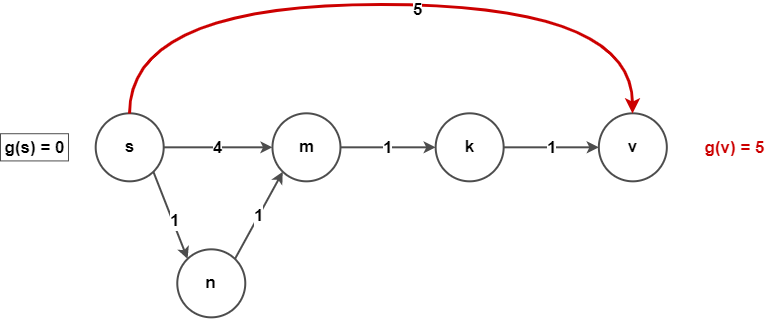
\includegraphics[width=0.8\linewidth]{img/incorrect_g1}
		\caption{Gráf korrektségének elromlása 1.}
		\label{fig:incorrect_gone}
	\end{figure}

    \noindent Elindulunk az $s$ startcsúcsból. Tekintve, hogy a gráfkeresés nem terjeszt ki rosszabb csúcsot, így az $s \rightarrow m \rightarrow k$ úton a $k$ csúcsot már nem terjeszti ki, mert $\pi(m)=s$ esetén $g(v) = 6 > 5 \ \textit{(eddig talált legrövidebb út)}$.\\

	\begin{figure}[H]
		\centering
        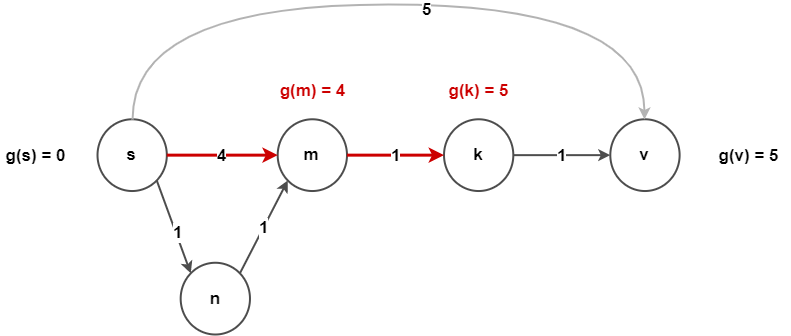
\includegraphics[width=0.8\linewidth]{img/incorrect_g2}
		\caption{Gráf korrektségének elromlása 2.}
		\label{fig:incorrect_gtwo}
	\end{figure}

    \noindent A $\pi(m) = n$ esetén a $g(m)=2$ azonban a gráf korrektsége nem megfelelő, mivel a korábban eltárolt $g(v)=5$ és $g(k)=5$ értékek már nem helyesek.

	\begin{figure}[H]
		\centering
        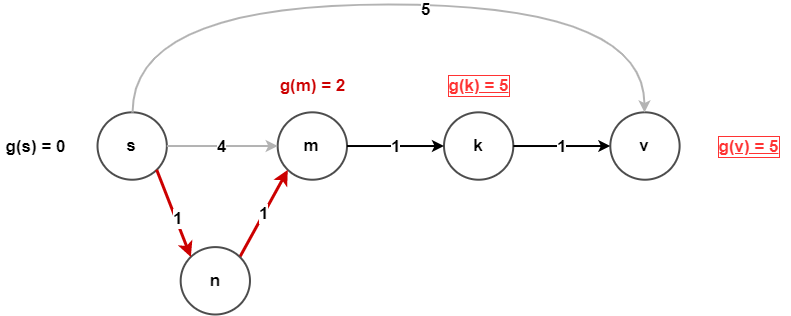
\includegraphics[width=0.8\linewidth]{img/incorrect_g3}
		\caption{Gráf korrektségének elromlása 3.}
		\label{fig:incorrect_gthree}
	\end{figure}

    \newpage
    \section*{Nevezetes gráfkereső algoritmusok}

    \newcolumntype{L}{>{\arraybackslash}m{7cm}}

    \subsection*{Nem informált gráfkereső algoritmusok}

    \noindent Azokat a keresőket, melyek az aktuális állapotról csak annyit tudnak, hogy célállapot-e, nem informált keresési algoritmusoknak nevezzük.\\
    {\small
    \renewcommand{\arraystretch}{2}
        \begin{tabular}{ l|c|L }
          \makecell{\\{\footnotesize \textit{\textbf{Mélységi gráfkeresés}}}\\\\\adjincludegraphics[valign=M,width=0.4\textwidth]{img/melysegi_graf_ker}\\ {\footnotesize {\color{white}$\triangle$}}} & \makecell{$f = -g$ \\ $\forall (n,m)$ élre\\$c(n,m)=1$} &
          \begin{tabular}[c]{L}
             - végtelen gráfokban csak mélységi korláttal garantál megoldást\\
             - {\scriptsize {\color{blue} \faLightbulbO\ $\triangleright$} a vizsgált reprezentációs gráf minden élének súlyát egységnyinek tekinti, és a kiértékelő függvénye az egyes csúcsokba vezető útköltségnek, az algoritmus által számolt g függvény értékének mínusz egyszerese, azaz f = –g. Egységnyi élsúlyok esetén a g költségfüggvény egy csúcsban a startcsúcsból odavezető már megtalált út hosszúságát mutatja, így a –g kiértékelés mindig a startcsúcstól legtávolabb eső, a legmélyebben fekvő nyílt csúcs kiterjesztését részesíti előnyben. (Azonos mélységű csúcsok esetén véletlenszerűen, vagy valamilyen másodlagos szempont alapján dönt.) Ezt a keresést gyakran egy mélységi korláttal is ellátják, így ha létezik a mélységi korlátnál nem hosszabb megoldási út, akkor a keresés megoldás megtalálásával terminál.$\triangleleft$ \faLightbulbO}
          \end{tabular}
          \\ \hline
          \makecell{\\{\footnotesize \textit{\textbf{Szélességi gráfkeresés}}}\\\\\adjincludegraphics[valign=M,width=0.4\textwidth]{img/szelessegi_graf_ker}\\ {\footnotesize {\color{white}$\triangle$}}} & \makecell{$f = g$\\$c(n,m)=1$} &
                           \begin{tabular}[c]{L}
                                  - optimális megoldást ad, ha van (még végtelen $\delta$ gráfban is)\\
                                  - egy csúcs kiterjesztésekor ismeri az odavezető legrövidebb utat (legfeljebb egyszer terjeszt ki)
                            \end{tabular} \\ \hline
           \makecell{\\{\footnotesize \textit{\textbf{Egyenletes gráfkeresés}}}\\} & $f = g$ &
                           \begin{tabular}[c]{@{}L@{}}
                                  - optimális (legolcsóbb) megoldást ad, ha van (még végtelen $\delta$ gráfban is)\\
                                  - egy csúcs kiterjesztésekor ismeri az odavezető legolcsóbb utat (legfeljebb egyszer terjeszt ki)\\
                            \end{tabular}\\
        \end{tabular}
    \renewcommand{\arraystretch}{1}}

    \subsection*{Heurisztikus gráfkereső algoritmusok}
    
    \noindent Az MI problémák szempontjából azok a kiértékelő függvények az érdekesek, amellyek egy nyílt csúcs ígéretességének megítélésekor heurisztikus ismeretekre is támaszkodnak. A heurisztika a gráfkereső algoritmusoknál olyan függvény formájában fogalmazható meg, amelyik minden csúcsra megbecsüli annak a legolcsóbb útnak a költségét, amelyen az adott csúcsból célcsúcsba lehet eljutni. \emph{\textbf{Heurisztikus függvény}}nek nevezzük azt a $h:N \rightarrow \R$ függvényt, amelyik egy csúcsnál megbecsüli a csúcsból a célba vezető (,,hátralévő”) optimális út költségét.
    \begin{center}
      $h(n) \approx h^{*}(n)$, ahol $h^{*}:N \rightarrow \R$
    \end{center}
    A $h^{*}$ egy \emph{elméleti} költségfüggvény a hátralévő optimális költség $n$-ből a célcsúcsok valamelyikébe.\\\\
    \noindent \emph{Nevezetes tulajdonságai}:\\\\
    \renewcommand{\arraystretch}{2}
    \begin{tabular}{l|l|l}
       \textit{{Nem-negatív}} & $h(n) \geqq 0$ & $\forall n \in N$
       \\ \hline
       \textit{{Megengedhető}} & $h(n) \leqq h^{*}(n)$ & $\forall n \in N$ {\small \text{(nem becsüli túl az optimális költséget ($h^{*}$))}}
       \\ \hline
       \textit{{Monoton megszorítás}} & $h(n)-h(m) \leqq c(n,m)$ & $\forall (n,m) \in A$
    \end{tabular}
    \renewcommand{\arraystretch}{1}\\\\

    \noindent \textbf{Definíció.} Egy gráfkereső algoritmus kiértékelő függvényét \emph{csökkenőnek} nevezzük akkor, ha egy nyílt csúcs kiértékelő függvényértéke csak akkor változik meg és akkor is csak csökken, ha az eddiginél olcsóbb utat találunk hozzá.\\

    \noindent \textbf{Tétel}. Egy csökkenő kiértékelő függvényt használó GK soha nem terjeszt inkorrekt csúcsot.\\
    \newpage
    \noindent \textbf{Heurisztikus keresést használó algoritmusok}\\
    \renewcommand{\arraystretch}{2}
        \begin{tabular}{ l|c|L }
           \textit{Előre tekintő gráfkeresés}       & $f = h$ &
                            \begin{tabular}[c]{@{}L@{}}
                                  - sikeres terminálást nem garantál\\
                                  - eredményessége és hatékonysága erősen függ a heurisztikus függvénytől
                            \end{tabular}
           \\ \hline
           \textit{\textbf{A} algoritmus}       & \makecell{$f = g+h$\\ $h \geq 0$} & - megoldást ad, ha van
           \\ \hline
           \textit{\textbf{A}* algoritmus}      & \makecell{$f = g+h$\\ $h^* \geqq h \geq 0$} & - optimális megoldást ad, ha van
           \\ \hline
           \textit{\textbf{A}$^C$ algoritmus}   & \makecell{$f = g+h$\\ $h^* \geq h \geq 0$\\\\ $\forall (n,m)$ élre\\ $h(n)-h(m) \leq c(n,m)$} &
                           \begin{tabular}[c]{@{}L@{}}
                                  - optimális megoldást ad, ha van\\
                                  - {\scriptsize {\color{blue} \faLightbulbO\ $\triangleright$} A monoton tulajdonság a heurisztikus függvény által adott becslés következetességére utal. Ilyenkor ugyanis nem fordulhat elő az, hogy a heurisztika rossznak látná a cél elérésének esélyét egy olyan csúcsból, amelynek kis költségű lépéssel elért utódcsúcsából már hirtelen igen ígéretesnek tartana $\triangleleft$ \faLightbulbO}\\
                                  - egy csúcs kiterjesztésekor ismeri az odavezető legolcsóbb utat\\
                                  - legfeljebb egyszer terjeszt ki
                            \end{tabular}
           \\ \hline
           \textit{\textbf{B} algoritmus}      & \makecell{$f = g+h$\\ $h \geq 0$ \\ + belső kiértékelő függvény $g$} & - a $g$-t használjuk a kiterjesztendő csúcs kiválasztására azon nyílt csúcsok közül, amelyek $f$ értéke kisebb, mint az eddig kiterjesztett csúcsok $f$ értékeinek maximuma.\\
        \end{tabular}
    \renewcommand{\arraystretch}{1}\\\\

    \noindent Véges $\delta$-gráfokon minden gráfkeresés terminál, és ha van megoldás, talál egyet. A nevezetes gráfkeresések többsége végtelen nagy gráfokon is találnak megoldást, ha van megoldás. (Kivétel az előre-tekintő keresés és a mélységi korlátot nem használó mélységi gráfkeresés.)\\

    \noindent Egy gráfkeresés memória igényét a kiterjesztett csúcsok számával, futási idejét ezek kiterjesztéseinek számával mérjük. (Egy csúcs általában többször is kiterjesztődhet, de $\delta$-gráfokban csak véges sokszor.)\\

    \noindent $A$* algoritmusnál a futási idő legrosszabb esetben exponenciálisan függ a kiterjesztett csúcsok számától, de ha olyan heurisztikát választunk, amelyre már $A^C$ algoritmust kapunk, akkor a futási idő lineáris lesz. Persze ezzel a másik heurisztikával változik a kiterjesztett csúcsok száma is, így nem biztos, hogy egy $A^C$ algoritmus ugyanazon a gráfon összességében kevesebb kiterjesztést végez, mint egy csúcsot többször is kiterjesztő A* algoritmus.\\

    \noindent A $B$ algoritmust tehát mindig érdemes az $A^*$ algoritmus helyett alkalmazni, ha a heurisztikánk nem monoton, mert a megvalósítása alig tér el az $A^*$ algoritmustól, eredményessége és memória igénye azonos vele, de a futási ideje jóval gyorsabb is lehet, lassabb viszont soha.
\newpage
	\section*{Kétszemélyes (teljes információjú, zéró összegű, véges) játékok}

    \noindent Egy játék leírásához a következőket kell megadni:
    \begin{itemize}
        \item A játék lehetséges állásait (helyzeteit).
        \item A játékosok számát.
        \item Hogyan következnek/lépnek az egyes játékosok (pl. egy időben vagy felváltva egymás után).
        \item Egy-egy állásban a játékosoknak milyen lehetséges lépései (lehetőségei) vannak.
        \item A játékosok milyen -- a játékkal kapcsolatos -- információval rendelkeznek a játék folyamán.
        \item Van-e a véletlennek szerepe a játékban és hol.
        \item Milyen állásban kezdődik és mikor ér véget a játék.
        \item Az egyes játékosok mikor, mennyit nyernek, illetve veszítenek.
    \end{itemize}

    \subsubsection*{Osztályozás}

    \begin{itemize}
        \item A játékosok száma szerint: pl. egy-, két-, \emph{\textbf{n-személyes}} játékok.
        \item Ha a játszma állásból állásba vivő lépések sorozata \emph{\textbf{diszkrét}} a játék.
        \item Ha az állásokban véges sok lehetséges lépése van minden játékosnak és a játszmák véges sok lépés után véget érnek \emph{\textbf{véges}} a játék.
        \item Ha a játékosok a játékkal kapcsolatos összes információval rendelkeznek a játék folyamán,\\
        \emph{\textbf{teljes információjú}} a játék.
        \item Ha nincs a véletlennek szerepe a játékban, \emph{\textbf{determinisztikus}} a játék.
        \item A játékosok nyereségeinek és veszteségeinek összege 0, akkor \emph{\textbf{zérusösszegű}} a játék.\\
    \end{itemize}
    
    \noindent A továbbiakban játék alatt kétszemélyes, diszkrét, véges, teljes információjú, determinisztikus, zérusösszegű játékot értünk.

    \subsubsection*{Játékfa}
   	
    \noindent A játékokat állapottér-reprezentációval szokás leírni, és az állapot-gráfot faként ábrázolják.\\\\
    {\small
    \renewcommand{\arraystretch}{2}
        \begin{tabular}{ l|L }
           \textit{\textbf{csúcs}}  & állás (egy állás több csúcs is lehet)
           \\ \hline
           \textit{\textbf{szint}}  & játékos (felválltva A és B szintjei)
           \\ \hline
           \textit{\textbf{él}}     & lépés (szintről-szintre)
           \\ \hline
           \textit{\textbf{gyökér}} & kezdő állás (kezdő játékos)
           \\ \hline
           \textit{\textbf{levél}}  & végállások
           \\ \hline
           \textit{\textbf{ág}}     & játszma
           \\
        \end{tabular}
    \renewcommand{\arraystretch}{1}}\\

    \subsection*{Nyerő stratégia}
    \begin{itemize}
    	\item A \textit{győztes (vagy nem-vesztes) stratégia} egy olyan elv, amelyet betartva egy játékos az ellenfél minden lépésére tud olyan választ adni, hogy megnyerje (ne veszítse el) a játékot. Valamelyik játékosnak biztosan van győztes (nem-vesztes) stratégiája.
        \item Győztes (nem-vesztes) stratégia keresése a \textit{játékfában} kombinatorikus robbanást okozhat, ezért e helyett részfa kiértékelést szoktak alkalmazni a soron következő jó lépés meghatározásához.
        \item A két esélyes (győzelem vagy vereség) teljes információjú véges determinisztikus kétszemélyes játékokban az egyik játékos számára biztosan létezik nyerő stratégia.
        \item A három esélyes játékokban (van döntetlen is) a nem vesztő stratégiát lehet biztosan garantálni.
    \end{itemize}

    \noindent \textbf{ÉS/VAGY gráf}
    \begin{itemize}
    \item A játék az egyik játékos szempontjából egy ÉS/VAGY fával ábrázolható.
    \begin{itemize}
        \item saját szinten egy csúcs utódai között VAGY kapcsolat van
        \item ellenfél szintjén egy csúcs utódai között ÉS kapcsolat van
    \end{itemize}
    \item A nyerő (nem-vesztő) stratégiát az ÉS/VAGY játékfa azon hiper-útja mutatja, amely a gyökércsúcsból csupa nyerő (nem-vesztő) levélcsúcsba vezet.
    \item A nyerő stratégia keresése tehát egy ÉS/VAGY fa beli hiper-út keresési probléma.
    \end{itemize}

    \subsection*{Algoritmusok}

    \noindent A nyerő vagy nem-vesztő stratégia megkeresése egy nagyobb játékfa esetében reménytelen. Az optimális lépés helyett a soronkövetkező jó lépést keressük (\emph{részleges játékfa-kiértékelés}). \\

    \noindent Ehhez az aktuális állapotból indulva kell a játékfa
    \begin{enumerate}
        \item néhány szintjét felépíteni,
        \item ezen a részfa leveleinek a hasznosságát megbecsülni,
        \item majd a soron következő lépést meghatározni.
    \end{enumerate}
    Minden esetben szükségünk van egy olyan heurisztikára, amely a mi szempontunkból becsüli meg egy állás hasznosságát.\\

    \subsubsection*{Minimax \emph{algoritmus}}

    \begin{enumerate}
        \item A játékfának az adott állás csúcsából leágazó részfáját felépítjük néhány szintig.
        \item A részfa leveleit kiértékeljük a kiértékelő függvény segítségével.
        \item Az értékeket felfuttatjuk a fában:
        \begin{itemize}
            \item A saját ($MAX$) szintek csúcsaihoz azok gyermekeinek maximumát:
            \begin{center}
                szülő := max\Big($gyerek_1,\ \ldots \,\ gyerek_k$\Big)
            \end{center}
            \item Az ellenfél (MIN) csúcsaihoz azok gyermekeinek minimumát:
            \begin{center}
                szülő := min\Big($gyerek_1,\ \ldots\ ,\ gyerek_k$\Big)
            \end{center}
            \item Soron következő lépésünk ahhoz az álláshoz vezet, ahonnan a gyökérhez felkerült a legnagyobb érték
        \end{itemize}
    \end{enumerate}
    
   \newpage
        {\color{mygray}
   \noindent Az algoritmust minden alkalommal megismételjük valahányszor mi következünk. Lehetséges, hogy az ellenfél nem feltétlenül az általunk várt legerősebb lépésekkel válaszol, mert:
        \begin{itemize}
          \item eltérő mélységű részfával dolgozik,
          \item más kiértékelő függvényt használ,
          \item nem minimaxeljárást alkalmaz,
          \item hibázik.\\
        \end{itemize}
        }
	
    \begin{figure}[H]
		\centering
        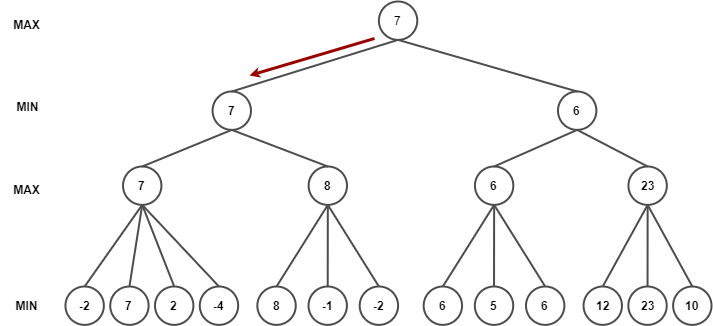
\includegraphics[width=0.8\linewidth]{img/minmax_sample.png}
		\caption{Minimax algoritmus példa.}
		\label{fig:minmax_sample}
	\end{figure}

    \noindent A $\ref{fig:minmax_sample}$. ábrán csak azt jelöljük, hogy melyik részfán indul el a játékos, mivel csak azt tudjuk, hogy merre kedvezőbb elindulnia. Az előző felsorolás alapján nem garantált, hogy végig is tudja játszani az adott pillanatban számára optimális játékot.

    \subsubsection*{Alfa-Béta \emph{algoritmus}}
    \begin{itemize}
    \item Visszalépéses algoritmus segítségével járjuk be a részfát (olyan mélységi bejárás, amely mindig csak egy utat tárol).\\
    Az aktuális úton fekvő csúcsok ideiglenes értékei:
    \begin{itemize}
        \item A $MAX$ szintjein $\alpha$ érték: ennél rosszabb értékű állásba innen már nem juthatunk
        \item A $MIN$ szintjein $\beta$ érték: ennél jobb értékű állásba onnan már nem juthatunk
    \end{itemize}
    \item Lefelé haladva a fában $\alpha:= -\infty$, és $\beta:= +\infty$.
    \item Visszalépéskor az éppen elhagyott (gyermek) csúcs értéke (\emph{felhozott érték}) módosíthatja a szülő csúcs értékét:
    \begin{itemize}
        \item A $MAX$ szintjein: $\alpha:= max\Big(\textit{felhozott érték},\ \alpha\Big)$
        \item A $MIN$ szintjein: $\beta:= min\Big(\textit{felhozott érték},\ \beta\Big)$
    \end{itemize}
    \item Vágás történik, ha az úton van olyan $\alpha$ és $\beta$, hogy $\alpha\ \geq\ \beta$.\\
    \end{itemize}
    \newpage
    Példa:\\

    \begin{figure}[H]
		\centering
        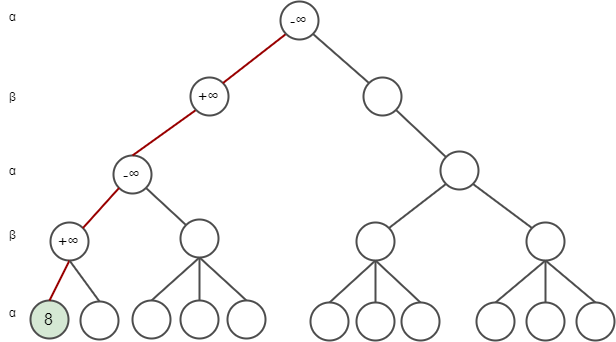
\includegraphics[width=0.72\linewidth]{img/alphabeta_01.png}
		\caption{Alfa-Béta algoritmus példa.}
		\label{fig:alphabetaone}
	\end{figure}

    \begin{figure}[H]
		\centering
        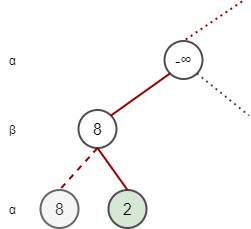
\includegraphics[width=0.32\linewidth]{img/alphabeta_02.png}
        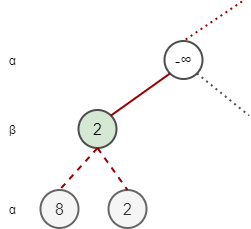
\includegraphics[width=0.32\linewidth]{img/alphabeta_03.png}
        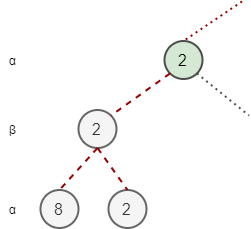
\includegraphics[width=0.32\linewidth]{img/alphabeta_04.png}
		\caption{Alfa-Béta algoritmus példa.}
		\label{fig:alphabetatwo}
	\end{figure}

    \begin{figure}[H]
		\centering
        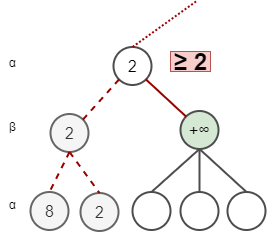
\includegraphics[width=0.32\linewidth]{img/alphabeta_05.png}
        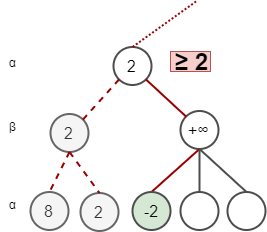
\includegraphics[width=0.32\linewidth]{img/alphabeta_06.png}
        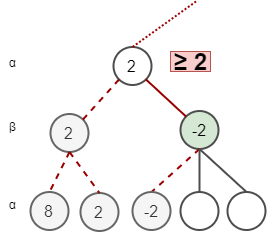
\includegraphics[width=0.32\linewidth]{img/alphabeta_07.png}
		\caption{Alfa-Béta algoritmus példa.}
		\label{fig:alphabetathree}
	\end{figure}

    \noindent A vágás a $\ref{fig:alphabetafour}$. ábra első képen a MIN ($\beta$) ágon történik. Mivel az ellenfél szempontjából a $-2$ jobb érték, mint a bal oldali részfán már megtalált $2$-es érték, ezért a MAX algoritmus használó játékos nem választaná ezt az ágat. Ennek oka, hogy az ellenfél szempontjából kedvezőbb ,,lépést" tartalmaz. Ezért nem számít, hogy a részfa maradék (még meg nem vizsgált) levelei között lenne nagyobb érték a $2$-nél.

    \begin{figure}[H]
		\centering
        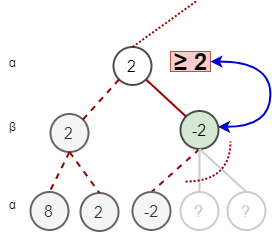
\includegraphics[width=0.32\linewidth]{img/alphabeta_08.png}
        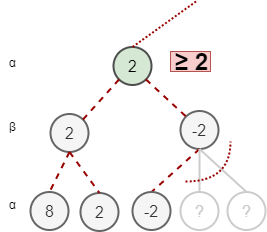
\includegraphics[width=0.32\linewidth]{img/alphabeta_09.png}
        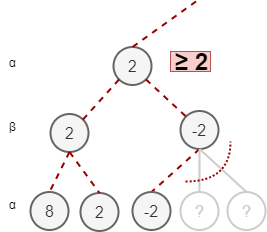
\includegraphics[width=0.32\linewidth]{img/alphabeta_10.png}
		\caption{Alfa-Béta algoritmus példa.}
		\label{fig:alphabetafour}
	\end{figure}

    \begin{figure}[H]
		\centering
        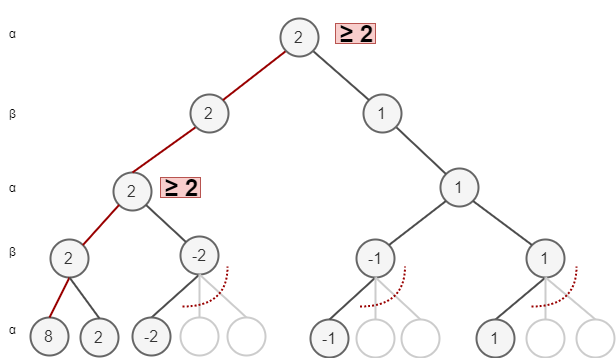
\includegraphics[width=0.72\linewidth]{img/alphabeta_end.png}
		\caption{Alfa-Béta algoritmus példa.}
		\label{fig:alphabetaend}
	\end{figure}

    \noindent Az algoritmus hatékonyságát az adja, hogy nagy problématér esetén rengeteg számítástól kíméli meg az algoritmust használó programot, így csökkentve a válaszidőt. Például egy sakk program esetén ki kell értékelni az egyes állásokat. Ez általában úgy történik, hogy konstans értéket rendel a program az egyes , ami már használható az algoritmusban. Ehhez például a sakkban konstans értékeket rendelhetünk az egyes figurákhoz. Majd egyes állásokat a megmaradt figurák összértéke alapján értékelhetünk.

    \begin{figure}[H]
		\centering
        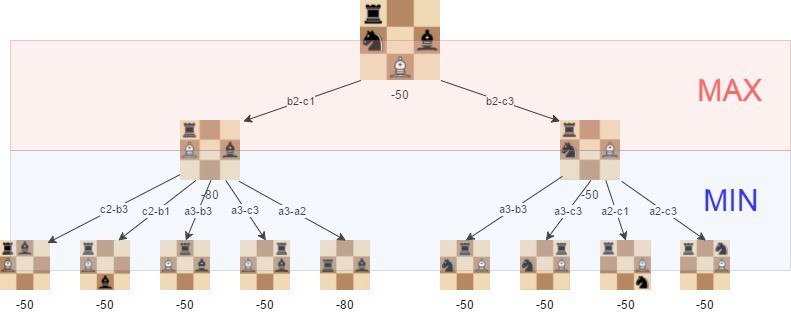
\includegraphics[width=0.65\linewidth]{img/chess_minmax.jpeg}
		\caption{Sakk példa: lépés keresés (Minimax).}
		\label{fig:minmaxchess}
	\end{figure}

    \begin{figure}[H]
		\centering
        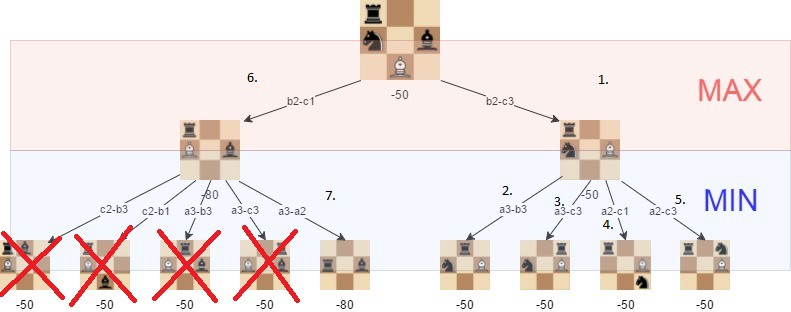
\includegraphics[width=0.65\linewidth]{img/chess_alphabeta.jpeg}
		\caption{Sakk példa: lépés keresés (Alfa-Béta).}
		\label{fig:alphabetachess}
	\end{figure}

    \noindent A $\ref{fig:alphabetachess}$. ábrán látható, hogy az Alpha-Beta algoritmussal megspórolunk rengeteg időt azzal, hogy az egyes állásokhoz tartozó konstans értéket nem szükséges kiszámítanunk.\\

	\subsubsection*{A \emph{Minimax} algoritmus további módosításai}

        \begin{itemize}
            \item \textbf{\emph{Átlagoló}}: Kisimítja a kiértékelő függvény esetleges tévedéseit.
            \begin{itemize}
                \item MAX szintre az $m$ darab legnagyobb értékű gyerek átlaga,
                \item MIN szintre az $n$ darab legkisebb értékű gyerek átlaga kerül.
            \end{itemize}
            \begin{figure}[H]
		      \centering
                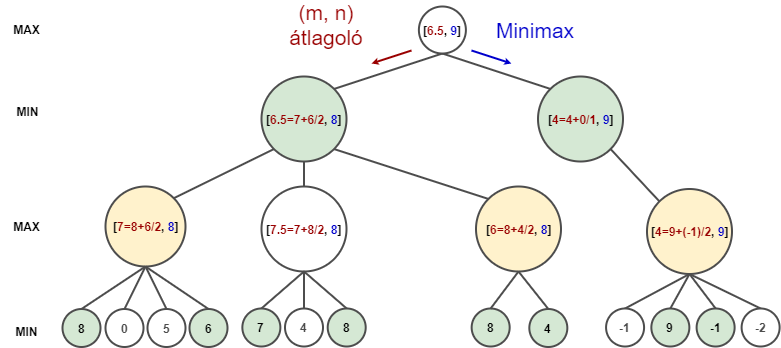
\includegraphics[width=0.8\linewidth]{img/avgminmax_sample.png}
		      \caption{Átlagoló kiértékelésű Minimax.}
		      \label{fig:avgminmax}
	       \end{figure}
            \item \textbf{\emph{Váltakozó mélységű kiértékelésű}}: A kiértékelő függvény minden ágon reális értéket mutat.\\
            Egy adott szintig (minimális mélység) mindenképpen felépítjük a részfát, majd ettől a szinttől kezdve egy másik adott szintig (maximális mélység) csak azon csúcsok gyerekeit állítjuk elő, amelyek még nincsenek nyugalomban, amelyre nemteljesül a nyugalmi teszt:
                \begin{center}
                $\Big|\ f(\textit{szülő})\ ‒\ f(\textit{csúcs})\ \Big|\ <\ K$\\
                \end{center}
            \begin{figure}[H]
		      \centering
                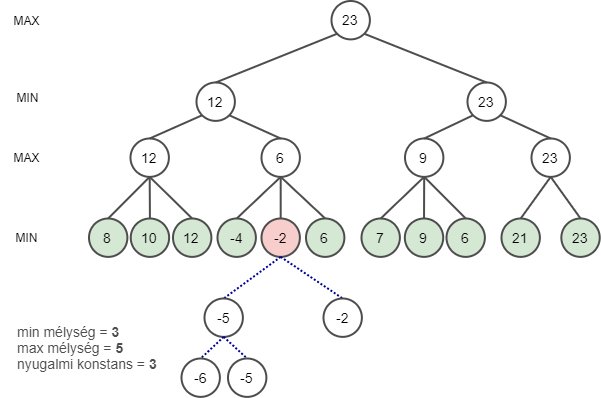
\includegraphics[width=0.8\linewidth]{img/variable_depth_minmax.png}
		      \caption{Vátozó mélységű kiértékelésű Minimax.}
		      \label{fig:avgminmax}
	       \end{figure}
            \item \textbf{\emph{Negamax}}: A Negamax eljárást könnyebb implementálni.
            \begin{itemize}
                \item Kezdetben (‒1)-gyel szorozzuk azon levélcsúcsok értékeit, amelyek az ellenfél (MIN) szintjein vannak, majd
                \item Az értékek felfuttatásánál minden szinten az alábbi módon számoljuk a belső csúcsok értékeit:
                \begin{center}
                    $\textit{szülő := max}\Big(\ ‒gyerek_1,\ \ldots\ ,\ ‒gyerek_k\ \Big)$
                \end{center}
            \end{itemize}
            \begin{figure}[H]
		      \centering
                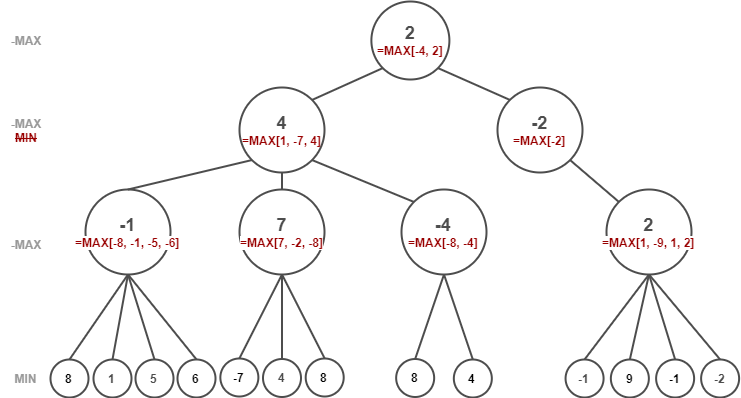
\includegraphics[width=0.8\linewidth]{img/negamax_sample.png}
		      \caption{Negamax algoritmus példa.}
		      \label{fig:negamax}
	       \end{figure}
    \end{itemize}	

\end{document} 